\subsection{Normalized Angular Velocity Input}
The Castle Creations ESC incorporates a microcontroller that employs a
nonlinear scaling mechanism to transform the input PWM (Pulse-width modulation) signal's duty cycle
($u_p$) into the duty cycle of the $24,kHz$ PWM signals sent to the inverter,
thereby effectively adjusting the source voltage applied to the
motor\cite{kim2017electric}. This non-linear transformation aims to achieve a
linear input-to-thrust relationship for intuitive manual operation.
Consequently, the PWM input to the ESC ($u_p$) undergoes filtering through a
non-linear function, denoted as $g_u$, resulting in the PWM duty-cycle input to
the inverter ($u$). This relationship can be represented as:
%===
\begin{align}\label{eqn::esc_input}
    u &= g_u(u_p), \qquad
    V_s = u V_{in} \qquad u \in [0, 1]
\end{align}
\begin{align*}
\text{Where,}\qquad&\\
    V_s &- \text{Effective voltage to the motor (lumped)}\\
    V_{in} &- \text{Battery voltage}
\end{align*}
%===
A constant PWM switching frequency of $400 \, Hz$ is utilized. The current ESC
equipped with RPM feedback capabilities operates within the range of $1110 \,
\mu s$ to $1890 \, \mu s$ of PWM duty-cycles. Beyond this range, the ESC
switches to a constant power mode, maintaining a constant RPM.

It's worth noting that the specific parameters governing the non-linear filter are not ascertainable with the available information. Consequently, neither $u_m$ nor $u_p$ can be considered the true input for system identification in conjunction with the propeller. To circumvent this issue, we redefine the input as the motor's angular velocity with the propeller, normalized by the input voltage ($u_\omega$). We then establish a static mapping between this quantity and the PWM input to the ESC ($u_p$).

In the steady-state condition ($\dot \omega = 0$), (\ref{eqn:dyn_mdl}) simplifies to:
%===
\begin{align}
    &\frac{b_m}{K_r} \left(\frac{\omega_m}{V_{in}}\right) + \frac{V_{in}}{K_r} C_D \lr{\frac{\omega}{V_{in}}}^2 + \frac{M_f}{K_r V_{in}} = u
\end{align}
%===
We introduce a term, $u_{\omega}$, which represents the angular velocity of the motor with the propeller at unit supply voltage for the given PWM input ($u_p$). This is termed as "\textit{Normalized Angular Velocity}".
%===
\begin{align}
    u_{\omega} &= \frac{\omega}{V_{in}} \text{  at  } u = g_u(u_p) \\
    \implies u &= \underbrace{\frac{b_m}{K_r} u_\omega + \frac{\hat V_{in}}{K_r} C_D u_\omega^2 + \frac{M_f}{K_r  \hat V_{in}}}_{g_\omega (u_\omega, \hat V_{in})}
     \label{eqn::input_def}
\end{align}
where $\hat V_{in}$ is the battery voltage at calibration $(15.54\,V)$.
%===
The relationship between $u_\omega$ and $u_p$ can be estimated from the static
measurement data (Fig.-\ref{fig::norm_omega}).
%===
\begin{figure}[H]
    \centering
    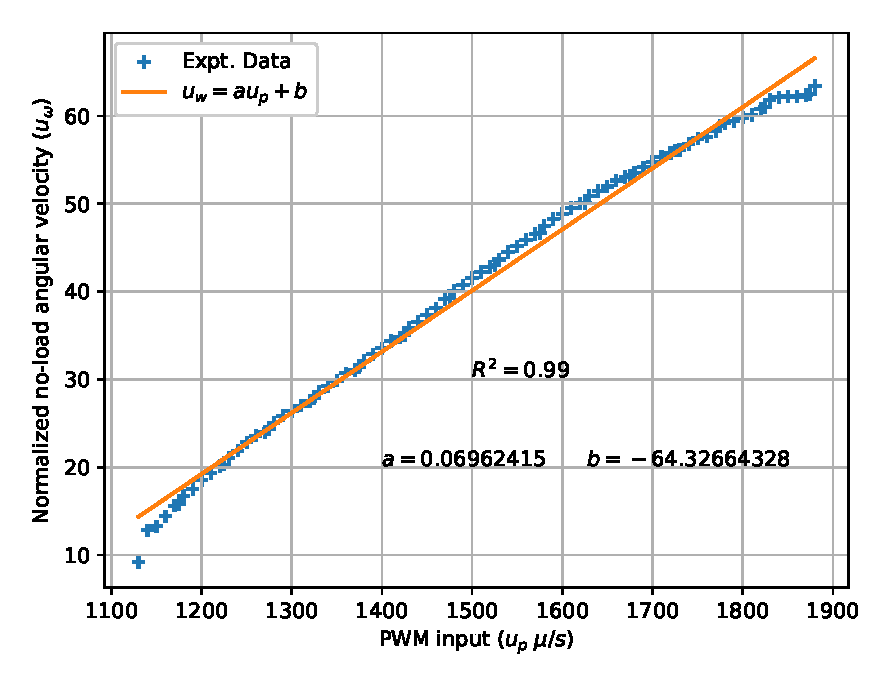
\includegraphics[width = 0.49\textwidth]{Part2/figs/3_figs/norm_omega/no-load_rpm.eps}
    \caption{$u_\omega$ as a function of $u_p$}
    \label{fig::norm_omega}
\end{figure}
%===
\begin{align}
    &u_\omega = a u_p + b
    \quad a = 0.0696
    \quad b = -64.3266\\
    \implies& g_u(u_p) = g_\omega(a u_p  + b, \hat V_{in})
    \; [\because u = g_\omega(u_\omega, \hat V_{in})]
\end{align}
